% https://www.essayempire.co.uk/complete-guide-about-the-structure-of-a-term-paper

\documentclass[a4paper, 10pt, english]{extarticle}
% %%%%%%%%%%%%%%%%%%%%%%% Code highlighting %%%%%%%%%%%%%%%%%%%%%%%%
\usepackage{minted} % Has to be the main document to work inline.
\usemintedstyle{mani}
% %%%%%%%%%%%%%%%%%%%%%%%%%%%%%%%%%%%%%%%%%%%%%%%%%%%%%%%%%%%%%%%%%%

% %%%%%%%%%%%%%%%%%%%%%%%%%%%%%% Layout %%%%%%%%%%%%%%%%%%%%%%%%%%%%%
\usepackage{geometry} % Customize page layout
\geometry{verbose,tmargin=2.0cm,bmargin=2.5cm,lmargin=2.0cm,rmargin=2.5cm}
% \parindent=0pt % Turns off paragraph indentation.
% \usepackage[paper=portrait,pagesize]{typearea}
% \usepackage{lscape}
\usepackage{multicol, multirow} % For multiple columns and rows.
\usepackage{fancyhdr} % Fancy headers and footers
\usepackage{lastpage} % references the number of pages in the document
% %%%%%%%%%%%%%%%%%%%%%%%%%%%%%%%%%%%%%%%%%%%%%%%%%%%%%%%%%%%%%%%%%%

% %%%%%%%%%%%%%%%%%%%%%%%%%%%%% Text %%%%%%%%%%%%%%%%%%%%%%%%%%%%%%%
\usepackage[utf8]{inputenc}
\usepackage[english]{babel} % Language support
\usepackage[parfill]{parskip} % Sets full justification and paragraph spacing
% \usepackage{setspace}
% \onehalfspacing % this is what the final report should be to improve readability
% \doublespacing % you may want to use this for drafts to your supervisor as it provides more space for comments
\usepackage[normalem]{ulem} % Underlining text.
\usepackage{soul,color} % emphasizing and highlighting text parts
% \usepackage{enumitem} % Customize enumerate, itemize and description
\usepackage[autostyle]{csquotes} % Quotation support
\MakeOuterQuote{"} %prevents backwards quote symbols
\usepackage{lipsum}
% %%%%%%%%%%%%%%%%%%%%%%%%%%%%%%%%%%%%%%%%%%%%%%%%%%%%%%%%%%%%%%%%%%

% %%%%%%%%%%%%%%%%%%%%%%%%%%%%%% Links %%%%%%%%%%%%%%%%%%%%%%%%%%%%%
\usepackage[hidelinks]{hyperref} % Hides boxes around hyperlinked URLs
\usepackage{url} % Processes urls and add hyperlinks
\usepackage{doi} % hyperlinks DOI's in refs
% %%%%%%%%%%%%%%%%%%%%%%%%%%%%%%%%%%%%%%%%%%%%%%%%%%%%%%%%%%%%%%%%%%

% %%%%%%%%%%%%%%%%%%%%%%%%%%% Referencing %%%%%%%%%%%%%%%%%%%%%%%%%%
% \usepackage{cite} % Improved handling of numeric citations
\usepackage[round]{natbib} % Bibliography and citation styles
\setcitestyle{authoryear}

% ############################ Biblatex ############################
% % Define the bibliography file and the style apa.
% %APA style guide: https://ctan.uib.no/macros/latex/contrib/biblatex-contrib/biblatex-apa/biblatex-apa-test.pdf
% %%\autocite - Within a paragraph, not in the narrative sense: (Koehler, 2016)
% %\textcite - Koehler (2016)
% \usepackage[style=apa,backend=biber]{biblatex}
% \DeclareLanguageMapping{british}{british-apa}
% \addbibresource{references.bib}
% ##################################################################

\usepackage{chngcntr}
\counterwithin{figure}{section} % Labels figures using the section number rather than continuous numbering
\usepackage[nottoc]{tocbibind} % Adds the bibliography to the table of contents
\usepackage{listings}  % Provides a listings environment. USE: \listoffigures, \listoftables
% %%%%%%%%%%%%%%%%%%%%%%%%%%%%%%%%%%%%%%%%%%%%%%%%%%%%%%%%%%%%%%%%%%

% %%%%%%%%%%%%%%%%%%%%%%%%%%%% Math %%%%%%%%%%%%%%%%%%%%%%%%%%%%%%
% NOTE! Both used for matrices.
\usepackage{amsmath} % AMS mathematical facilities for LATEX.
\usepackage{mathtools} % extension package to amsmath, typesetting, allignment, etc,.
% %%%%%%%%%%%%%%%%%%%%%%%%%%%%%%%%%%%%%%%%%%%%%%%%%%%%%%%%%%%%%%%%%%

% %%%%%%%%%%%%%%%%%%%%%%%%%%%% Tables %%%%%%%%%%%%%%%%%%%%%%%%%%%%%%
\usepackage[table,xcdraw]{xcolor} % colors, tints, shades, tones.
\usepackage{tabularx} % Tables with adjustable width columns.
\usepackage{booktabs} % Fancy tables
% %%%%%%%%%%%%%%%%%%%%%%%%%%%%%%%%%%%%%%%%%%%%%%%%%%%%%%%%%%%%%%%%%%

% %%%%%%%%%%%%%%%%%%%%%%%%%%%% Figures %%%%%%%%%%%%%%%%%%%%%%%%%%%%%
\usepackage{graphicx} % To see figures.
\usepackage{float} % Preventing latex re-positioning tables, include H.
\usepackage{wrapfig}  % Allows text wrapping around figures.
\usepackage{subfig}   % used for sub-figures
\usepackage{tikz}
\usepackage{tikz-uml} % To make UML Diagrams. NOTE! Needs yikz-uml.sty.
\usetikzlibrary{automata, positioning} % To make diagrams.
% %%%%%%%%%%%%%%%%%%%%%%%%%%%%%%%%%%%%%%%%%%%%%%%%%%%%%%%%%%%%%%%%%%

% %%%%%%%%%%%%%%%%%%%% Variables for Title Page %%%%%%%%%%%%%%%%%%%%
\newcommand\university{Noroff University College}
\newcommand\myCourseName{Course Name}
\newcommand\myCourseCode{Cource Code}
\newcommand\myTitle{Title}
\newcommand\myUndertitle{Undertitle}
\newcommand\myAuthorFirst{Lewi Lie}
\newcommand\myAuthorLast{\textsc{Uberg}}
\newcommand\myProfessorFirst{Dr. Gene}
\newcommand\myProfessorLast{\textsc{Rick}}
\newcommand\myLecturerFirst{Dr. Miscell}
\newcommand\myLecturerLast{\textsc{Aneous}}
\newcommand\myDate{\today}
% %%%%%%%%%%%%%%%%%%%%%%%%%%%%%%%%%%%%%%%%%%%%%%%%%%%%%%%%%%%%%%%%%%

% %%%%%%%%%%%%%%%%%%%%%% Variables for Title %%%%%%%%%%%%%%%%%%%%%%%
\author{\myAuthorFirst{} \myAuthorLast}
\title{\myTitle}
\date{\myDate}
% \makeatletter
% \renewcommand\@author{\myAuthorFirst{} \myAuthorLast}
% \renewcommand\@title{\myTitle}
% \renewcommand\@date{\myDate}
% \makeatother
% %%%%%%%%%%%%%%%%%%%%%%%%%%%%%%%%%%%%%%%%%%%%%%%%%%%%%%%%%%%%%%%%%%

% %%%%%%%%%%%%%%%%%%%%%%%%%%%% Header %%%%%%%%%%%%%%%%%%%%%%%%%%%%%%
% %%% Use with \pagestyle{fancy} %%%
%\lhead{\myCourseCode\\\myAuthorFirst{} \myAuthorLast}
%\rhead{\leftmark}

% %%% Use for custom \fancypagestyle{} %%%
% Fancyhdr Styles
\fancypagestyle{nomatter}{%
   \fancyhf{} % clear all fields
   \renewcommand{\headrulewidth}{0pt}
   \renewcommand{\footrulewidth}{0pt}
%   \lhead{\myCourseCode\\\myAuthorFirst{} \myAuthorLast}
%   \lfoot{}
%   \cfoot{}
%   \rfoot{}
}

\fancypagestyle{tocmatter}{%
   \fancyhf{} % clear all fields
   \renewcommand{\headrulewidth}{0.4pt} % add the footer horizontal line, default is 0pt
   \renewcommand{\footrulewidth}{0.4pt}
   \lhead{\myCourseCode\\\myAuthorFirst{} \myAuthorLast}
   \rhead{\leftmark}
%   \lfoot{}
%   \cfoot{}
%   \rfoot{}
}

\fancypagestyle{listmatter}{%
   \fancyhf{} % clear all fields
   \renewcommand{\headrulewidth}{0.4pt} % add the footer horizontal line, default is 0pt
   \renewcommand{\footrulewidth}{0.4pt}
   \lhead{\myCourseCode\\\myAuthorFirst{} \myAuthorLast}
   \rhead{\leftmark}
%   \lfoot{}
    \cfoot{\thepage}
%   \rfoot{}
}

\fancypagestyle{mainmatter}{%
   \fancyhf{} % clear all fields
   \renewcommand{\headrulewidth}{0.4pt} % add the footer horizontal line, default is 0pt
   \renewcommand{\footrulewidth}{0.4pt}
   \lhead{\myCourseCode\\\myAuthorFirst{} \myAuthorLast}
   \rhead{\leftmark}
%   \fancyhead[R]{\nouppercase{\leftmark}}
%   \lfoot{}
    \cfoot{\thepage\ of \pageref{LastPage}} % Add Page X of Y to the footer
%   \rfoot{}
}
% %%%%%%%%%%%%%%%%%%%%%%%%%%%%%%%%%%%%%%%%%%%%%%%%%%%%%%%%%%%%%%%%%%

% %%%%%%%%%%%%%%%%%%%%%%%%%%%%%%%%%%%%%%%%%%%%%%%%%%%%%%%%%%%%%%%%%%
% %%%%%%%%%%%%%%%%%%%%%%%%%%%%%%%%%%%%%%%%%%%%%%%%%%%%%%%%%%%%%%%%%%
% %%%%%%%%%%%%%%%%%%%%%%%%%%%%%%%%%%%%%%%%%%%%%%%%%%%%%%%%%%%%%%%%%%
\begin{document}

% %%%%%%%%%%%%%%%%%%%%%%%%%% If title page %%%%%%%%%%%%%%%%%%%%%%%%%
\begin{titlepage} %Prevents page numbering and inclusion in page count.
\newcommand{\HRule}{\rule{\linewidth}{.5mm}} % Defines a custom command.

\center
\textsc{\LARGE \university}\\[15mm]
\textsc{\Large \myCourseName}\\[5mm]
\textsc{\large \myCourseCode}\\[5mm]

\HRule\\[5mm]
{\huge\bfseries \myTitle}\\[5mm]
{\LARGE\bfseries \myUndertitle}\\[5mm]

\HRule\\[15mm]

\begin{minipage}{0.4\textwidth}
	\begin{flushleft}
		\large
		\textit{Author}\\
		\myAuthorFirst{} \myAuthorLast
	\end{flushleft}
\end{minipage}
~
\begin{minipage}{0.4\textwidth}
	\begin{flushright}
		\large
		\textit{Professor}\\
		\myProfessorFirst{} \textsc{\myProfessorLast}
	\end{flushright}
	\begin{flushright}
		\large
		\textit{Lecturer}\\
		\myLecturerFirst{} \textsc{\myLecturerLast}
	\end{flushright}
\end{minipage}

\vfill

\begin{figure}[H]
    \centering
    \includegraphics[width=0.5\textwidth]{Noroff.pdf}
\end{figure}

\vfill

%Made static when submitting 
{\large\myDate}

\end{titlepage}

% \pagenumbering{gobble}
\newpage

%\renewcommand{\footrulewidth}{0.4pt} % add the footer horizontal line, default is 0pt
%\pagestyle{fancy} %add fancy headers and footers

\pagenumbering{roman} %set page numbering to roman numerals
\pagestyle{tocmatter}
\setcounter{tocdepth}{3} % Controls the depth of contents
\tableofcontents

\newpage
\setcounter{page}{1}
\pagestyle{listmatter}
\listoffigures

\newpage
\pagestyle{listmatter}
\listoftables

\newpage
\renewcommand\listoflistingscaption{List of Source Codes}
\addcontentsline{toc}{section}{List of Source Codes}
\pagestyle{listmatter}
\listoflistings

\newpage
\setcounter{page}{1}
\pagestyle{mainmatter}
\pagenumbering{arabic} % Sets page number to digits
% %%%%%%%%%%%%%%%%%%%%%%%%%%%%%%%%%%%%%%%%%%%%%%%%%%%%%%%%%%%%%%%%%%

% %%%%%%%%%%%%%%%%%%%%%%%% If not title page %%%%%%%%%%%%%%%%%%%%%%%
% \maketitle
% %%%%%%%%%%%%%%%%%%%%%%%%%%%%%%%%%%%%%%%%%%%%%%%%%%%%%%%%%%%%%%%%%%

% \section*{Abstract} %the * says do not give a number
\begin{abstract}
\noindent
    A concise and factual abstract is required. The abstract should state briefly the purpose of the research, the principal results and major conclusions. An abstract is often presented separately from an article, so it must be able to stand alone. For this reason, references should be avoided. Also, non-standard or uncommon abbreviations should be avoided, but if essential they must be defined at their first mention in the abstract itself. The abstract is a short summary of your document as a whole. It is always suggested that your abstract should not be longer that 150 words.
    
    \bigskip %give some spacing between the abstract and keywords
    
    \textbf{{Keywords:}} \textit{Immediately after the abstract, provide a list of 5-10 keywords. Be sparing with abbreviations: only abbreviations firmly established in the field may be eligible. These keywords will be used for indexing purposes. Try \textbf{not} to use overly generic terms such as \textbf{Cyber Security}, \textbf{Digital Forensics}, or \textbf{Data Science}}
    
\end{abstract}


\section{Introduction}

% This is the first paragraph
This is the first \textbf{paragraph}. The number one occurs quite often in this paragraph. I am labelling every paragraph with their number, with this being one.

% This is the second paragraph
This is now the second \textit{paragraph}.
% Comments inside the paragraph. Since there is no blank line, it says one paragraph.
I am using this text to indicate that we are now in the second paragraph.

% This is the third paragraph
Lastly, I am also writing the third and final \underline{paragraph}. Three paragraphs is all we need for this example. This is teaching you \LaTeX{} in three easy paragraphs. But with additional packages, we can \xout{not} do more.

\subsection{This is a subsection with bullet-points}
\begin{itemize}
    \item Item One
    \item Item Two
\end{itemize}{}

\subsection{This is a subsection with enumeration}
\begin{enumerate}
    \item Item One
    \item Item Two
\end{enumerate}

\section{Mathematics in LaTeX}

You can write mathematics inline in three different ways. The first way is $E=mc^2$, The second way is \(E=mc^2\), and the last way is \begin{math}E=mc^2\end{math}.\newline
This illustrates how you can write the equation on their own line. This looks a lot better.
\[E=mc^2\]
The above mentioned way is not used often, as it is better to have your equations numbered. The typical way maths is shown when it is numbered is as follows. \begin{equation}
    E=mc^2
\end{equation}{}

\noindent
There are also other ways where mathematics is much easier to write in \LaTeX{}. We write integrals using $\int$ and fractions using $\frac{a}{b}$.
\begin{equation}
    \int_0^1 \frac{1}{e^x} = \frac{e-1}{e}
\end{equation}

Lower case Greek letters are written as $\omega$ $\delta$ etc. While upper case Greek letters are written as $\Omega$ $\Delta$

Mathematical operators are prefixed with a backslash as $\sin(\beta)$, $\cos(alpha)$, $\log(x)$ etc.

\section{Explaining Figures}
Figures are one of the most complicated items in \LaTeX{}. Similar to all other things in \LaTeX{}, a figure has to begin and end somewhere. We will also need to upload the figure. The preferred format for \LaTeX{} is PDF or TIFF files.

\begin{figure}[H]
    \centering
    \includegraphics[width=0.5\textwidth]{Noroff.pdf}
    \caption{Noroff Logo}
    \label{fig:noroff_logo}
\end{figure}

As you can see in figure \ref{fig:noroff_logo}, this is the logo you encounter every time you are browsing social media. Figure \ref{fig:noroff_logo} is used by Noroffs marketing team even on page \pageref{fig:noroff_logo}.

\section{Explaining Tables}
Table are quite difficult to draw in \LaTeX{}, however, it is something that is needed quite often. Lets start by doing a very basic table.

\begin{table}[H]
    \centering
    \begin{tabular}{c c c}
    cell1 & cell2 & cell3 \\
    cell4 & cell5 & cell6 \\
    cell7 & cell8 & cell9
    \end{tabular}
    \caption{Test table 1}
    \label{tab:test_table1}
\end{table}

There is a table, however, it does not look like a normal table. We are missing the lines. Let's add the lines to it now.

\begin{table}[H]
    \centering
    \begin{tabular}{| c | c | c |}
    \hline
    cell1 & cell2 & cell3 \\
    cell4 & cell5 & cell6 \\
    cell7 & cell8 & cell9 \\
    \hline
    \end{tabular}
    \caption{Test table 2}
    \label{tab:test_table2}
\end{table}

\bigbreak

The last table, table \ref{tab:test_table3}, depicts the students at NUC that are sick of the online marketing campaign. There are many different ways how we can design it.
Something to note, the caption on a table is always \textbf{above} and the caption on a figure should always be \textbf{below} it.

\begin{table}[H]
    \centering
    \caption{Students marketing opinions}
    \begin{tabular}{|| c | c | c ||}
    \hline
    Location & Like & Dislike \\
    \hline
    \hline
    Oslo & 3 & 972 \\
    Kristiansand & 0 & 5486 \\
    Bergen & 1 & 875 \\
    \hline
    \hline
    Total & 4 & 7333 \\
    \hline
    \end{tabular}
    \label{tab:test_table3}
\end{table}

\subsection{Generating tables online}
% Please add the following required packages to your document preamble:
% \usepackage[table,xcdraw]{xcolor}
% If you use beamer only pass "xcolor=table" option, i.e. \documentclass[xcolor=table]{beamer}
% \usepackage[normalem]{ulem}
% \useunder{\uline}{\ul}{}
\begin{table}[H]
    \centering
    \caption{Using www.tablesgenerator.com}
    \begin{tabular}{lll}
    \hline
    \multicolumn{3}{|l|}{Merged Heading} \\ \hline
    {\color[HTML]{96FFFB} cell1} & \textbf{cell2} & \cellcolor[HTML]{32CB00}cell3 \\
    \textit{cell4} & \cellcolor[HTML]{CE6301}cell5 & {\ul cell6}
    \end{tabular}
\end{table}

\begin{table}[H]
    \centering
    \caption{Using www.latex-tables.com}
    \begin{tabular}{lll} 
    \hline
    \multicolumn{3}{|l|}{Merged Heading} \\ 
    \hline
    \textcolor{cyan}{cell1} & \textbf{cell2} & cell3 \\
    \textit{cell4} & cell5 & \uline{cell6} 
    \end{tabular}
\end{table}

\section{Booktabs}
\begin{table}[H]
    \centering
    \caption{Example of advanced tables}
    \medskip
    \small
    \begin{tabular}{lcccc}
        \toprule 
        Algorithm & KNN & DT  & LR & SVM \\ \midrule
        \rowcolor[gray]{.9} Accuracy in general & Medium & Medium & Medium & Good\\
        Explanation ability of the trained model & Good & Good & Medium & Low\\ 
        \rowcolor[gray]{.9} Model parameter handling & Low & High & Low & High \\ 
        Learning time with respect to number of samples and features & - & $\mathcal{O}(n^2 d)$ & $\mathcal{O}(n d)$ & $\mathcal{O}(n^2 d + n^3)$ \\ 
        \rowcolor[gray]{.9} Time to classify a test sample & $\mathcal{O}(k n d)$ & $\mathcal{O}(d)$ & $\mathcal{O}(d)$ & $\mathcal{O}(n_{sv}d)$   \\
        Tolerance to noise &  Low & Medium & Low & Medium \\
        \rowcolor[gray]{.9} Tolerance to overfitting & Medium & Low & Medium & High \\
        \multicolumn{5}{r}{n = number of observations ~~~~~} \\
        \multicolumn{5}{r}{d = number of features \,~~~~~~~~~~} \\
        \multicolumn{5}{r}{k = number of dimensions ~~~~~~} \\
        \multicolumn{5}{r}{$n_{sv}$ = number of support vectors} \\
        \bottomrule
    \end{tabular}
\end{table}

\newpage
\section{Multiple columns}
\begin{multicols}{2}
    \lipsum[1]
\end{multicols}

\section{Code highlighting}

% \renewcommand\listoflistingscaption{List of source codes}
% \listoflistings

\begin{listing}[H]
    \begin{minted}
    [
    frame=lines,
    %framesep=2mm,
    %baselinestretch=1.2,
    %bgcolor=lightgray,
    fontsize=\footnotesize,
    %linenos,
    mathescape,
    %rulecolor,
    %showspaces
    ]
    {python}
    import numpy as np
        
    def incmatrix(genl1,genl2):
        m = len(genl1)
        n = len(genl2)
        M = None #to become the incidence matrix
        VT = np.zeros((n*m,1), int)  #dummy variable
        
        #compute the bitwise xor matrix
        M1 = bitxormatrix(genl1)
        M2 = np.triu(bitxormatrix(genl2),1) 
    
        for i in range(m-1):
            for j in range(i+1, m):
                [r,c] = np.where(M2 == M1[i,j])
                for k in range(len(r)):
                    VT[(i)*n + r[k]] = 1;
                    VT[(i)*n + c[k]] = 1;
                    VT[(j)*n + r[k]] = 1;
                    VT[(j)*n + c[k]] = 1;
                    
                    if M is None:
                        M = np.copy(VT)
                    else:
                        M = np.concatenate((M, VT), 1)
                    
                    VT = np.zeros((n*m,1), int)
        
        return M
    \end{minted}
\caption{Example from internal code}
\label{listing:1}
\end{listing}

\noindent
\\
Testing One-line code.
\mint{python}|Lewi = [ letter for letter in 'Lewi' ]|

\newpage
\noindent
Testing from external file.

\begin{listing}[H]
\inputminted{python}{test_code.py}
\caption{Example from external file}
\label{listing:2}
\end{listing}

\noindent
Double backslashes or newline at the end of a line performs a line-break. \\ Like this text on a new line. The hfill + break can also be used \hfill \break Like this.
\\
\\*
Double backslashes and a asterisk at the end of a line performs a line-break without making it a new paragraph. %A paragraph should never end with a \newline or \\

\vspace*{50px}
\noindent
noindent before a line in a new paragraph makes it have no indentation.
With vspace I can control the space before and after a paragraph.
\vspace{20px}

\noindent hfil breaks the line \hfil in two. \\*
hspace 1cm makes a space \hspace{1cm} of exactly that width.

\begin{flushleft}
  This is some text that is to the left 
\end{flushleft}

\begin{center}
  This is some text that is centered 
\end{center}

\begin{flushright}
  This is some text that to the right 
\end{flushright}


\subsection{Testing diagrams}
Figure \ref{fig:dia1} shows \textbf{one} way of making a diagram.
\begin{figure}[H]
\centering
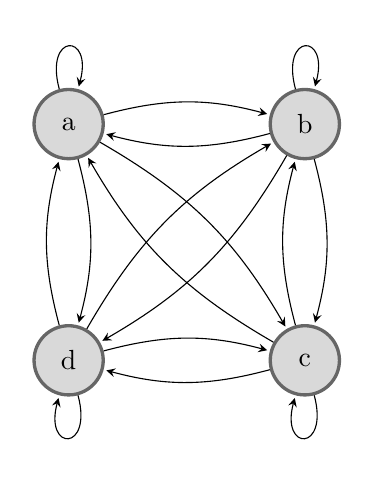
\begin{tikzpicture}%
  [>=stealth,
  shorten >=1pt,
  node distance=3cm,
  on grid,
  auto,
  every state/.style={draw=black!60, fill=black!15, very thick}
  ]
\node[state] (first)                        {a};
\node[state] (second)   [right=of first]    {b};
\node[state] (third)    [below=of second]   {c};
\node[state] (fourth)   [below=of first]    {d};

\path[->]
%   FROM    BEND/LOOP   POSITION OF LABEL   LABEL   TO
    (first) edge[loop above]    node {} (second)
            edge[bend left=15]  node {} (second)
            edge[bend left=15]  node {} (fourth)
            edge[bend left=15]  node {} (third)
    (second)edge[loop above]    node {} (first)
            edge[bend left=15]  node {} (third)
            edge[bend left=15]  node {} (first)
            edge[bend left=15]  node {} (fourth)
    (third) edge[loop below]    node {} (fourth)
            edge[bend left=15]  node {} (fourth)
            edge[bend left=15]  node {} (second)
            edge[bend left=15]  node {} (first)
    (fourth)edge[loop below]    node {} (first)
            edge[bend left=15]  node {} (first)
            edge[bend left=15]  node {} (third)
            edge[bend left=15]  node {} (second)
    ;
\end{tikzpicture}
\caption{Diagram One}
\label{fig:dia1}
\end{figure}

\noindent
Figure \ref{fig:dia2} shows \textbf{anoter} way of making a diagram.
\begin{figure}[H]
\centering
    \begin{tikzpicture}
    %%% Super Class %%%
    \umlclass{Client}{
    {\begin{tabular}{l r}
        client\_id : & int \\
        email : & str \\
        phone\_number : & int \\
        street\_name : & str \\
        street\_number : & str \\
        postal\_code : & int \\
        city : & str \\
        county : & str \\
        country : & str
    \end{tabular}}{}}{}
    
    %%% Child Class %%%
    \umlclass[x=-3, y=-4cm, anchor=north] {Persons}
    {\begin{tabular}{l r}%There are different ways of positioning the classes. "below left=4.5cm" Can be used for uniformly placement.
        first\_name : & str \\
        middle\_name : & str \\
        last\_name : & str \\
        social\_security\_number : & int
    \end{tabular}}{}
    
    %%% Child Class %%%
    \umlclass[x=3, y=-4cm, anchor=north] {Organizations}{
    {\begin{tabular}{l r}%Here I manually fine tune the positioning.
        organization\_name : & str \\
        organization\_number : & int
    \end{tabular}}{}}{}
    
    \umlVHVinherit[arm2=-3.25cm]{Persons}{Client}
    \umlVHVinherit[arm2=-3.25cm]{Organizations}{Client}
    %\umlVHVinherit[arg1=0..1, pos1=0.3]{Persons}{Client} ‰Not needed for inheritance
    %\umlVHVinherit[arg1=0..1, pos1=0.3, arg2=1, pos2=2.7]{Organizations}{Client} ‰Not needed for inheritance
    \end{tikzpicture}
\caption{Diagram Two}
\label{fig:dia2}
\end{figure}

\newpage
\section{The Matrix}
Here's a matrix in the center!
\[
\begin{matrix}
1 & 2 & 3 \\
4 & 5 & 6 \\
7 & 8 & 9
\end{matrix}
\]

Here's another matrix
$\begin{pmatrix}
1 & 2 & 3 \\
4 & 5 & 6 \\
7 & 8 & 9
\end{pmatrix}$
inline of the text.
\bigbreak

Here's the little brother
$\big(\begin{smallmatrix}
1 & 2 & 3 \\
4 & 5 & 6 \\
7 & 8 & 9
\end{smallmatrix}\big)$
inline of the text.
\bigbreak

Here's a matrix justified to the left.
\smallbreak
\begin{flushleft}
$\begin{bmatrix}
1 & 2 & 3 \\
4 & 5 & 6 \\
7 & 8 & 9
\end{bmatrix}$
\end{flushleft}
\bigbreak

Here's a matrix justified to the right.
\smallbreak
\begin{flushright}
$\begin{Bmatrix*}
1 & 2 & 3 \\
4 & 5 & 6 \\
7 & 8 & 9
\end{Bmatrix*}$
\end{flushright}
\bigbreak

Here's Johnny!
$\begin{vmatrix}
1 & 2 & 3 \\
4 & 5 & 6 \\
7 & 8 & 9
\end{vmatrix}$
\bigbreak

Here's Johnny's brother!
$\begin{Vmatrix}
1 & 2 & 3 \\
4 & 5 & 6 \\
7 & 8 & 9
\end{Vmatrix}$
\bigbreak

Here's Johnny's cousin!
$\left\lceil
\begin{matrix}
1 & 2 & 3 \\
4 & 5 & 6 \\
7 & 8 & 9
\end{matrix}
\right\rceil$
\bigbreak

Here's Johnny's baby momma!
$\left\lfloor
\begin{matrix}
1 & 2 & 3 \\
4 & 5 & 6 \\
7 & 8 & 9
\end{matrix}
\right\rfloor$
\bigbreak

Here's Johnny's sista!
$\left\langle
\begin{matrix}
1 & 2 & 3 \\
4 & 5 & 6 \\
7 & 8 & 9
\end{matrix}
\right\rangle$

\newpage
\section{Citation Test}
% \citet{key}	Jones et al. (1990)
% \citet*{key}	Jones, Baker, and Smith (1990)
% \citep{key}	(Jones et al. 1990)
% \citep*{key}	(Jones, Baker, and Smith 1990)
% \citep[p.~99]{key}	(Jones et al., 1990, p. 99)
% \citep[e.g.][]{key}	(e.g. Jones et al., 1990)
% \citep[e.g.][p.~99]{key}	(e.g. Jones et al., 1990, p. 99)
% \citeauthor{key}	Jones et al.
% \citeauthor*{key}	Jones, Baker, and Smith
% \citeyear{key}	1990
% \citeapos{key}*	Jones et al.'s (1990)
Making some citations outside brackets \cite{Bharathi.Sv2017} like this, and inside \citep{Bollen2010}, like this. We can include all author names \citep*{ElAlaoui2018}, like this. Or we can use et al. for more than two authors \citep{Kalyani2016}. We can even have multiple citations \citep{Kim2019}, like this. And finally we can include page numbers \citep[p.~22]{Kordonis2016}, like this.

\newpage
% \bibliographystyle{agsm} % Last name, then first letter of first name. DOI NOT INCLUDED
\bibliographystyle{abbrvnat} % First letter of first name, then last name.
% \bibliographystyle{plainnat} % Whole name.
\bibliography{references}

% %%%%%%%%%%%% For biblatex %%%%%%%%%%%%
% \printbibliography

\end{document}
